\section{Kostenwachstum je Release}
\label{sec:Kostenwachstum}

In einer Fallstudie hat \citeauth{martin2018} das Kostenwachstum für jedes erbrachte Release untersucht. Dabei hat er aus einem untersuchten Unternehmen, das anonym bleiben wollte, den Lebenszyklus eines marktführenden Softwareprodukts analysiert. Der Umfang des Entwicklungsteams hat über acht Releases signifikant zugenommen (\refAbb{fig:staff_rel}), die Anzahl der Zeilen an Quellcode hat sich ab einem gewissen Punkt aber nicht mehr stark vermehrt (\refAbb{fig:kloc_rel}). Die Produktivität des Entwicklerteams (\refAbb{fig:prod_rel}) fiel schon ab dem vierten Release mit jedem weiteren Release immer weiter gegen Null. Für das Entwicklerteam ist das frustrierend, da alle Bemühungen das Produkt zu erweitern, den Aufwand und die Anstrengungen für zukünftige Produktversionen vermehrt \citep[vgl.][5\psqq]{martin2018}. 

Bei der Analyse der Probleme ist \citeauth{martin2018} auf zwei wesentliche Faktoren gestoßen. Zum einen musste das Produkt schnell auf den Markt gebracht werden. Den Quellcode strukturieren und aufräumen könne aus Sicht der Projektleitungen danach erledigt werden und wurde entsprechend verschoben. Diese Vorgehensweise wurde aber weiterhin durchgeführt, da der Marktdruck nicht nachgelassen hat. Somit wurde die Wartung und Pflege des vorhandenen Quellcodes immer weiter aufgeschoben. Der andere Faktor war die Annahme, dass unordentlicher Code auf kurze Sicht einen Geschwindigkeitsvorteil bringt und alles andere langfristig nur aufhält \citep[vgl.][10]{martin2018}.

Der beste Weg die Lebensdauer von Softwareprodukten gewinnbringend zu erhöhen ist laut \citeauth{martin2018}, der Qualität der eigenen Softwarearchitektur mehr Bedeutung beizumessen und ernster zu nehmen \citep[vgl.][12]{martin2018}.


\begin{figure}
  \centering
  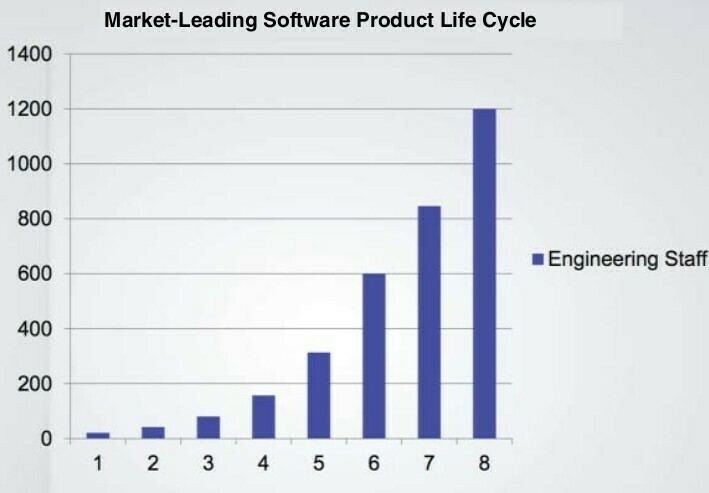
\includegraphics[width=.6\textwidth]{res/staff_releases.jpg}
   \caption{Personalwachstum im Entwicklungsbereich mit jedem Release \citep[][5]{martin2018}.}
   \label{fig:staff_rel}
\end{figure}


\begin{figure}
  \centering
  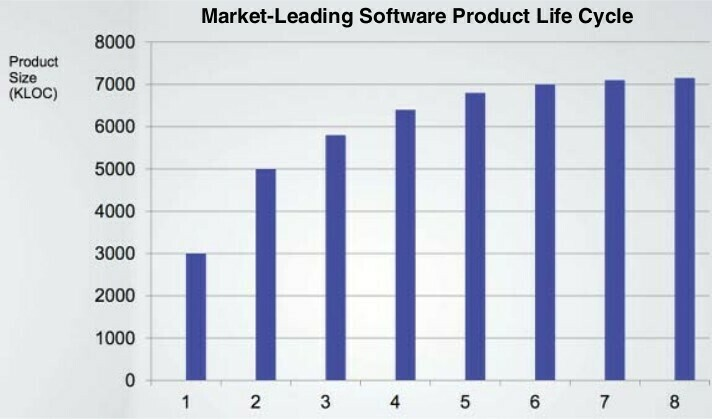
\includegraphics[width=.6\textwidth]{res/kloc_releases.jpg}
   \caption{Anzahl Zeilen an Quellcode mit jedem Release \citep[][6]{martin2018}.}
   \label{fig:kloc_rel}
\end{figure}


\begin{figure}
  \centering
  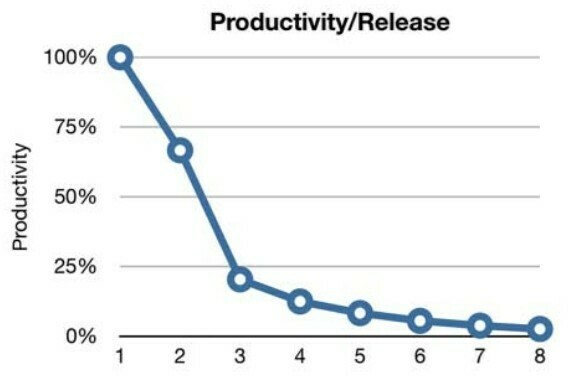
\includegraphics[width=.6\textwidth]{res/productivity_releases.jpg}
   \caption{Produktivität des Entwicklungsteams mit jedem Release \citep[][8]{martin2018}.}
   \label{fig:prod_rel}
\end{figure}


In einer weiteren Fallstudie setzt \citeauth{Ogheneovo2014} die Komplexität und die Instandhaltungs"= und Evolutionskosten von Software in Verbindung. Da Software sich über die Zeit weiter entwickelt (\textit{Evolution}), wird sie gleichzeitig auch komplexer, wenn nicht der Quellcode restrukturiert wird um die Komplexität zu verringern. Dies kann \zb als Ergebnis einer Instandhaltungsmaßnahme sein. Unter Evolution einer Software kann die Erweiterung von Funktionen verstanden werden, die einen weiteren Nutzerkreis ansprechen soll. Auch der Einsatz von neuen Technologien, um neuen Funktionen gerecht zu werden, fallen als Evolutionskosten an \citep[vgl.][3]{Ogheneovo2014}.

%\textquote[{\cite[][3]{Ogheneovo2014}}]{Software maintenance and evolution of systems was first proposed by Lehman in 1969 [11]. Lehman notes that systems continue to evolve over time. As a result, they become more complex unless some action such as code refactoring is adopted to reduce the complexity that may arise as a result of maintenance. [...] 
%The software value can be enhanced by expanding the customer base, meeting additional requirements, thus making the software more easier to use, more efficient, more reliable, and employing new technology to cater for the new features that may be introduced to these technologies. Software evolution plays an important role in software maintenance process. Most development effort and expenditure is allocated to the evolution and update of existing versions of software. Software is ceaselessly changed—maintained, evolved and updated—more often than it is written, and changing software is extremely costly.}.

In die Instandhaltungsphase fallen 60 bis 70\% der Aufwände. Damit umfasst sie den größten Teil der Entwicklung und auch einen Großteil der kompletten Lebenszykluskosten \citep[vgl.][3]{Ogheneovo2014}.

%\textquote[{\cite[][3]{Ogheneovo2014}}]{Barry et al. [14] notes that about 60 to 70\% effort is expended on maintenance phase of software development life cycle. It therefore suffix to say that software maintenance activities span a system’s productive life cycle and consume a major part of the total life cycle costs of the system. The software maintenance process can last for years or even decades after development process [15]. Therefore, there is need for effective planning in order to address the scope of software maintenance, the tailoring of the post delivery/deployment, the designation of who will pro- vide maintenance, and an estimation of the life-cycle costs. Software maintenance takes more effort than all the other phases of software life cycle.}.

Ein Faktor, der die Instandhaltungskosten verringern kann, ist die Modularisierung der Software. Hiermit werden Teile der Software in einzelne Module aufgeteilt und wieder neu miteinander verbunden. Durch die logische Aufteilung des Softwaredesigns kann die Komplexität verringert und die einzelnen Module wartbarer gemacht werden. In der Entwicklung spielt das Konzept der Modularisierung eine wichtige Rolle. \textit{Microsoft} hat mehr als drei Jahre gebraucht um \textit{Windows Vista} letztendlich zu veröffentlichen. Hier waren die Module logisch so groß aufgebaut, dass die Programmkomplexität anstieg. Mit jedem Patch und jeder Verbesserung wurde es schwieriger neue Funktionalitäten einzuführen. Deshalb mussten Untermodule geschaffen werden, welche die Komplexität verringerten. Durch die fehlende Strukturierung und Modularisierung des Programmcodes verzögerte sich die Markteinführung von \textit{Windows Vista} \citep[vgl.][8\psq]{Ogheneovo2014}.

%\textbf{Factors Affecting Software Maintenance Costs}
%\textquote[{\cite[][8\psq]{Ogheneovo2014}}]{Modularity: Modularity is the degree to which system’s components may be separated or recombined. In modular programming, modularity refers to the compartmentalization and inter-relation of the parts of a software system. It is the logical partitioning of software design that allows complex software to be manageable for the purpose of implementation and maintenance. This logic may be based on related functions, implementation considerations, data links etc. Baldwin and Clark [41] in their theory note that modular architectures add value to system designs by creating options to improve the system by substituting or experimenting on individual modules.
%The concept of modularity is very important in software development and maintenance. According to [42], it took Microsoft more than three years of delay before they finally released Windows Vista. This was attributed to the presence of large modules which made the software to increase program complexity. Therefore, for large modules to be meaningful and useful in a program, they must be broken down into smaller modules called sub-modules. Guth [43] opined that the delay was attributed to complexity resulting from the system’s lack of modularity. According to him, with each patch and enhancements, it became harder to strap new features into the software, since new code could affect everything else in unpredictable ways. This is why Walter [44] concluded that Microsoft Windows Vista is a 60-m- ines-of-code mess of spaghetti. This is because the code lacks pattern, is unstructured, and is not well modularized. Thus Microsoft suffered from unanticipated depen- dencies, modularity decay, and delays in bringing software to market. As seen from above, it is clear that there is no firm or organization that has been able to solve the problem of software complexity. According to Fried, even a firm with deep expertise in software development, like Microsoft, can still suffer from a complexity disaster resulting from a system’s lack of modularity.}.

Hier wurde auch festgestellt, dass mit jeder weiteren Version von Windows das Entwicklerteam immer weiter anwuchs. Von den Anwender*innen wurden mehr Funktionen gefordert, weswegen der Druck gewachsen ist die Deadline zu treffen. Aber je mehr Entwickler*innen an dem Code arbeiteten desto mehr Fehler entstanden \citep[vgl.][12]{Ogheneovo2014}.

%% --- MAYBE aber Übergang?--- %%
%\textquote[{\cite[][12]{Ogheneovo2014}}]{The table also shows that in each release of Windows version, the size of the development team is on the increase. This is because as more functionalities are needed by users, so there is pressure on the software  development team to release new products that will meet user’s demands and in the process of trying to meet deadlines, new maintainers will be employed and the more people are involved; the more bugs are introduced into the software. [...] It has been argued by some authors that SLOC is a poor productivity of individuals because developers can develop only a few lines and be more productive in terms of functionality than a developer who creates more lines of code which will eventually results in more effort both during development and maintenance phases. This is quite true. This is because inexperience programmers often result in code duplication which often makes the program lengthier and increase the lines of code which may even introduce new errors into the program. It could also cause the addition of dead codes, which may result in certain variables, parameters, functions, procedures, or methods, etc., not being used or referenced or called during the lifetime of the program.}.

\citeauth{Ogheneovo2014} kommt zu dem Schluss: \textquote[{\cite[][13]{Ogheneovo2014}}]{Complexity is a measure of understandability, and lack of understandability leads to errors}. Je komplexer ein System ist, desto schwieriger ist es zu spezifizieren, zu entwerfen, zu implementieren, zu verifizieren, zu bedienen und/oder zu ändern \citep[vgl.][13]{Ogheneovo2014}.

%\textquote[{\cite[][13]{Ogheneovo2014}}]{Complexity is a measure of understandability, and lack of understandability leads to errors. A system that is more complex may be harder to specify, harder to design, harder to implement, harder to verify, harder to operate, risky to change, and/or harder to predict its behavior. Complexity affects not only human understandability but also “machine understandability”. For example, static analysis tools for simple languages such as C are stronger than tools for more complex languages such as C++. Large and complex software projects require significant management control. They also introduce challenges as complex software systems are a crucial part of the organization. Also, the maintenance of large software systems requires a large number of employees. The estimated costs of software maintenance are high enough to justify strong efforts on the part of software managers to monitor and control complexity. Therefore, management must find ways to reduce the costs of software maintenance by ensuring that the right people are employed to maintain them to avoid more complication of the software.}.

Beide Fallstudien kommen also zu dem Schluss, dass eine hohe Komplexität die Wartung bestehender Software und dessen Evolution beeinträchtigt. Dies kann zu Verzögerungen in der Markteinführung neuer Funktionen oder einen erhöhten Kostenaufwand in der Entwicklung führen.


